
\documentclass[index]{subfiles}

\begin{document}
\doublespacing{}
\begin{titlepage}
   \begin{center}
       \vspace*{1cm}

       {\huge{Investigating the efficiency of Cheney stop-and-copy and LISP-2 mark-compact garbage collection algorithms}}

       \vspace{1.5cm}

       How does the runtime and collection performance of Cheney's stop-and-copy algorithm compare to the LISP-2 mark-compact algorithm?
            
       \vspace{1.5cm}

       \vfill
            
       International Baccalaureate Extended Essay\\
       jkv635\\

       \vspace{0.8cm}
     
       Computer science\\
       \vspace{0.8cm}
       Word Count: 3855\\
            
   \end{center}
\end{titlepage}

\addtocontents{toc}{\protect\thispagestyle{empty}}
\tableofcontents
\thispagestyle{empty}
\newpage
\setcounter{page}{1}

\section{Introduction}

Garbage collectors, and the algorithms they use, are incredibly widespread in just about any application one can find in the modern-day.

One example of these applications is their use in higher-level programming languages. Javascript is the only programming language of the web and drives the functionality of all web pages. Python is today's most popular and rising programming language and drives artificial intelligence development. Java, a still prevalent programming language, is used to make \textit{Minecraft}, one of the most popular games of the world, played by millions.

The element these languages all have in common is that they are interpreted languages, and they automatically manage memory by using garbage collectors.

It thus follows that the algorithms behind garbage collection and their relative efficiencies are ever more important to consider, now that more interpreted languages are being run on more and more devices over time. 

Contemporary research on the subject has become increasingly complex, factoring in new algorithms or combining old algorithms. Many assume the basic algorithms as known information and haven't tested simple algorithms on modern hardware.

This paper aims to shed light on the essential component of higher-level languages that many programmers tend to look over, presenting information in an easily digestible way, as well as applying that knowledge practically by implementing a simple stop-and-copy and mark-compact garbage collection algorithm in the same programming language and comparing their performance.

\subsection{Methodology}

To thoroughly compare and contrast the differences between these two algorithms and make an educated analysis of the results later, a basic understanding of how memory works in a program, the terminology concerning memory management, and the definition of garbage needs to be researched and understood.

First the basic steps in each algorithm will be researched. This includes when garbage collection is run, how live objects are determined, and what objects are moved where during the compaction process of each algorithm.

Next, the removal of garbage, as well as the access of garbage-collected data will be tested for each algorithm, and the time recorded.

Finally, research will be done on the basics of hardware caches and organization of memory in modern systems, and this information will be used to critically analyze the results of the performance of the two algorithms.

\section{Background}

The data of all computer programs are stored in a place we call memory. Whenever one wants to make room for new data, one must allocate memory to free space. And whenever one wants to remove data, one must deallocate that memory back into free space.

In modern computers, there are two places where the program can allocate memory: the stack and the heap~\parencite{the_rust_programming_language}.

Garbage collection is most concerned with the heap because this is where objects can be accessed at random and where objects with dynamic sizes (that is, sizes unknown at the time we compile our program) can be stored. In a running program, when there are dynamically sized objects expanding and decreasing in size and objects that are allocated but no longer in use, there needs to be a way to reclaim this memory automatically. Thus memory management aims to determine which parts of the heap are ``free'' memory and which sections are ``used'' memory.

\subsection{Memory Management Techniques}

There are several ways to manage memory in a language. One is by manually allocating and deallocating: the programmer specifies precisely how much memory is needed at a specific time and decides when something should be deallocated. In lower-level languages, this is normal. However, manual allocation often requires considerable experience to learn and increases the time required for developers to think about and write a program. It also easily results in many types of bugs, such as using memory that is already freed, freeing memory twice, and not freeing memory in the first place~\parencites{garbage_collection_overview_uw}[Chapter~1]{gc_handbook}

Hence, to alleviate the burden of keeping track of manual memory management, many modern programming languages use automatic memory management. There are many different ways to manage memory automatically. The only types of garbage collectors this paper is concerned with are tracing garbage collectors, which, as their name suggests, directly check objects to determine if they are ``alive'' (used by the program) or ``dead'' (not in use any longer)~\parencite{a_unified_theory_of_garbage_collection}. This is usually determined by traversing some tree of the live objects~\parencite[Chapter~1]{gc_handbook}, then declaring everything else garbage.

The central concept of garbage collection algorithms consists of just two steps. To create a new object, \verb+allocate()+is called, which calculates if there exists enough free space on the heap and occupies that section of memory. To free up memory the \verb+collect()+~\parencite{gc_handbook} function is called. This function finds all the live objects (and moves them, in the case of copying and compacting collectors) freeing other space. 

\subsection{LISP-2 Sliding Mark-Compact Algorithm}

One variant of the mark-compact garbage collector is the \textit{sliding} LISP-2 algorithm.

\begin{figure}[H]
    \centering
    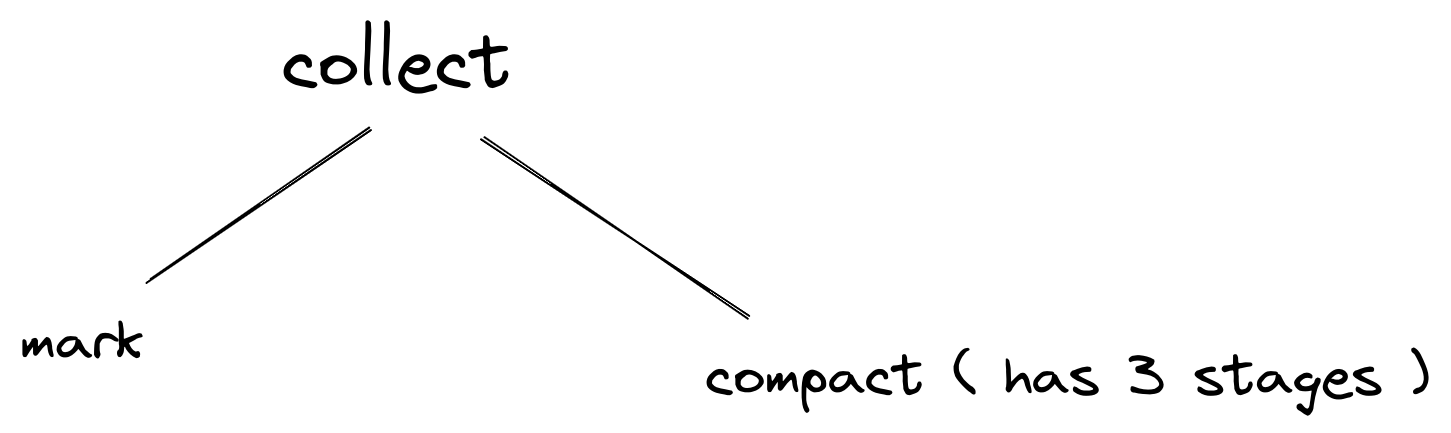
\includegraphics[scale=0.3]{pics/mark-compact-overview.png}
    \caption{Basic overview of mark-compact algorithm}
\end{figure}

The \verb+collect()+ consists of two stages. In the \verb+mark()+ stage, ``living'' objects are found, and in the \verb+compact()+ stage, a series of computations ``slide'' these living objects down to one end, compacting the heap in the process and freeing up space~\parencite[Chapter~3]{gc_handbook}.

\subsubsection{The Marking Stage}

To determine which objects are alive and dead, we attempt to traverse the entire heap through the graph of objects. We start from the root nodes, located on the stack~\parencites[Ch~3~Marking]{redhat_openjdk}[Chapter~3]{gc_handbook}, adding the objects that they reference to a worklist (which can either be a stack or a queue, to traverse breadth-first or depth-first). Then for every object in the worklist, we mark the object (if we haven't already), then add their children to the worklist. This action is iterated repeatedly until the worklist is exhausted. Accessible objects can eventually be reached by this recursion of reference from the roots. Objects that are then found to be inaccessible (because they are unmarked) are defined as `garbage' and can be ignored in the \verb+compact+ phase.

There are several ways to ``mark'' an object that is accessible~\parencite[Chapter~3]{gc_handbook}. A straightforward way is to mutate the object's specific, dedicated boolean field. This could be the same field as used for the forwarding address necessary for the compact stage as discussed later~\parencite[Chapter~1]{gc_handbook}.

\subsubsection{Compact Stage}

The compaction stage consists of three parts. In each, the heap is traversed in its entirety.

First, we calculate where the living object will slide down after copying. Start by initializing a \verb+free+ pointer starting at the very bottom of the heap. Then iterate over all the memory in the heap. For every object that is marked (which we determined by checking the \verb+forwarding_address+ field of each object we mutated), set the new address of the object in question to the free pointer, then bump the free pointer by the object's size~\parencites[Chapter~3]{gc_handbook}[Sections~3.3--3.5]{redhat_openjdk}. 

Second, we update the references of each marked living object to point to the new \verb+forwarding_address+ of where they'll eventually be moved. Iterate over the heap a 2nd time, only looking at marked objects again. Then for each reference (or it could be thought of as each ``child'' object that a ``parent'' object references), we retrieve the \verb+forwarding_address+ for that referenced object and set that as the new reference to the object~\parencites[Chapter 3]{gc_handbook}[Sec.~3.4]{redhat_openjdk}.

\begin{figure}[H]
    \centering
    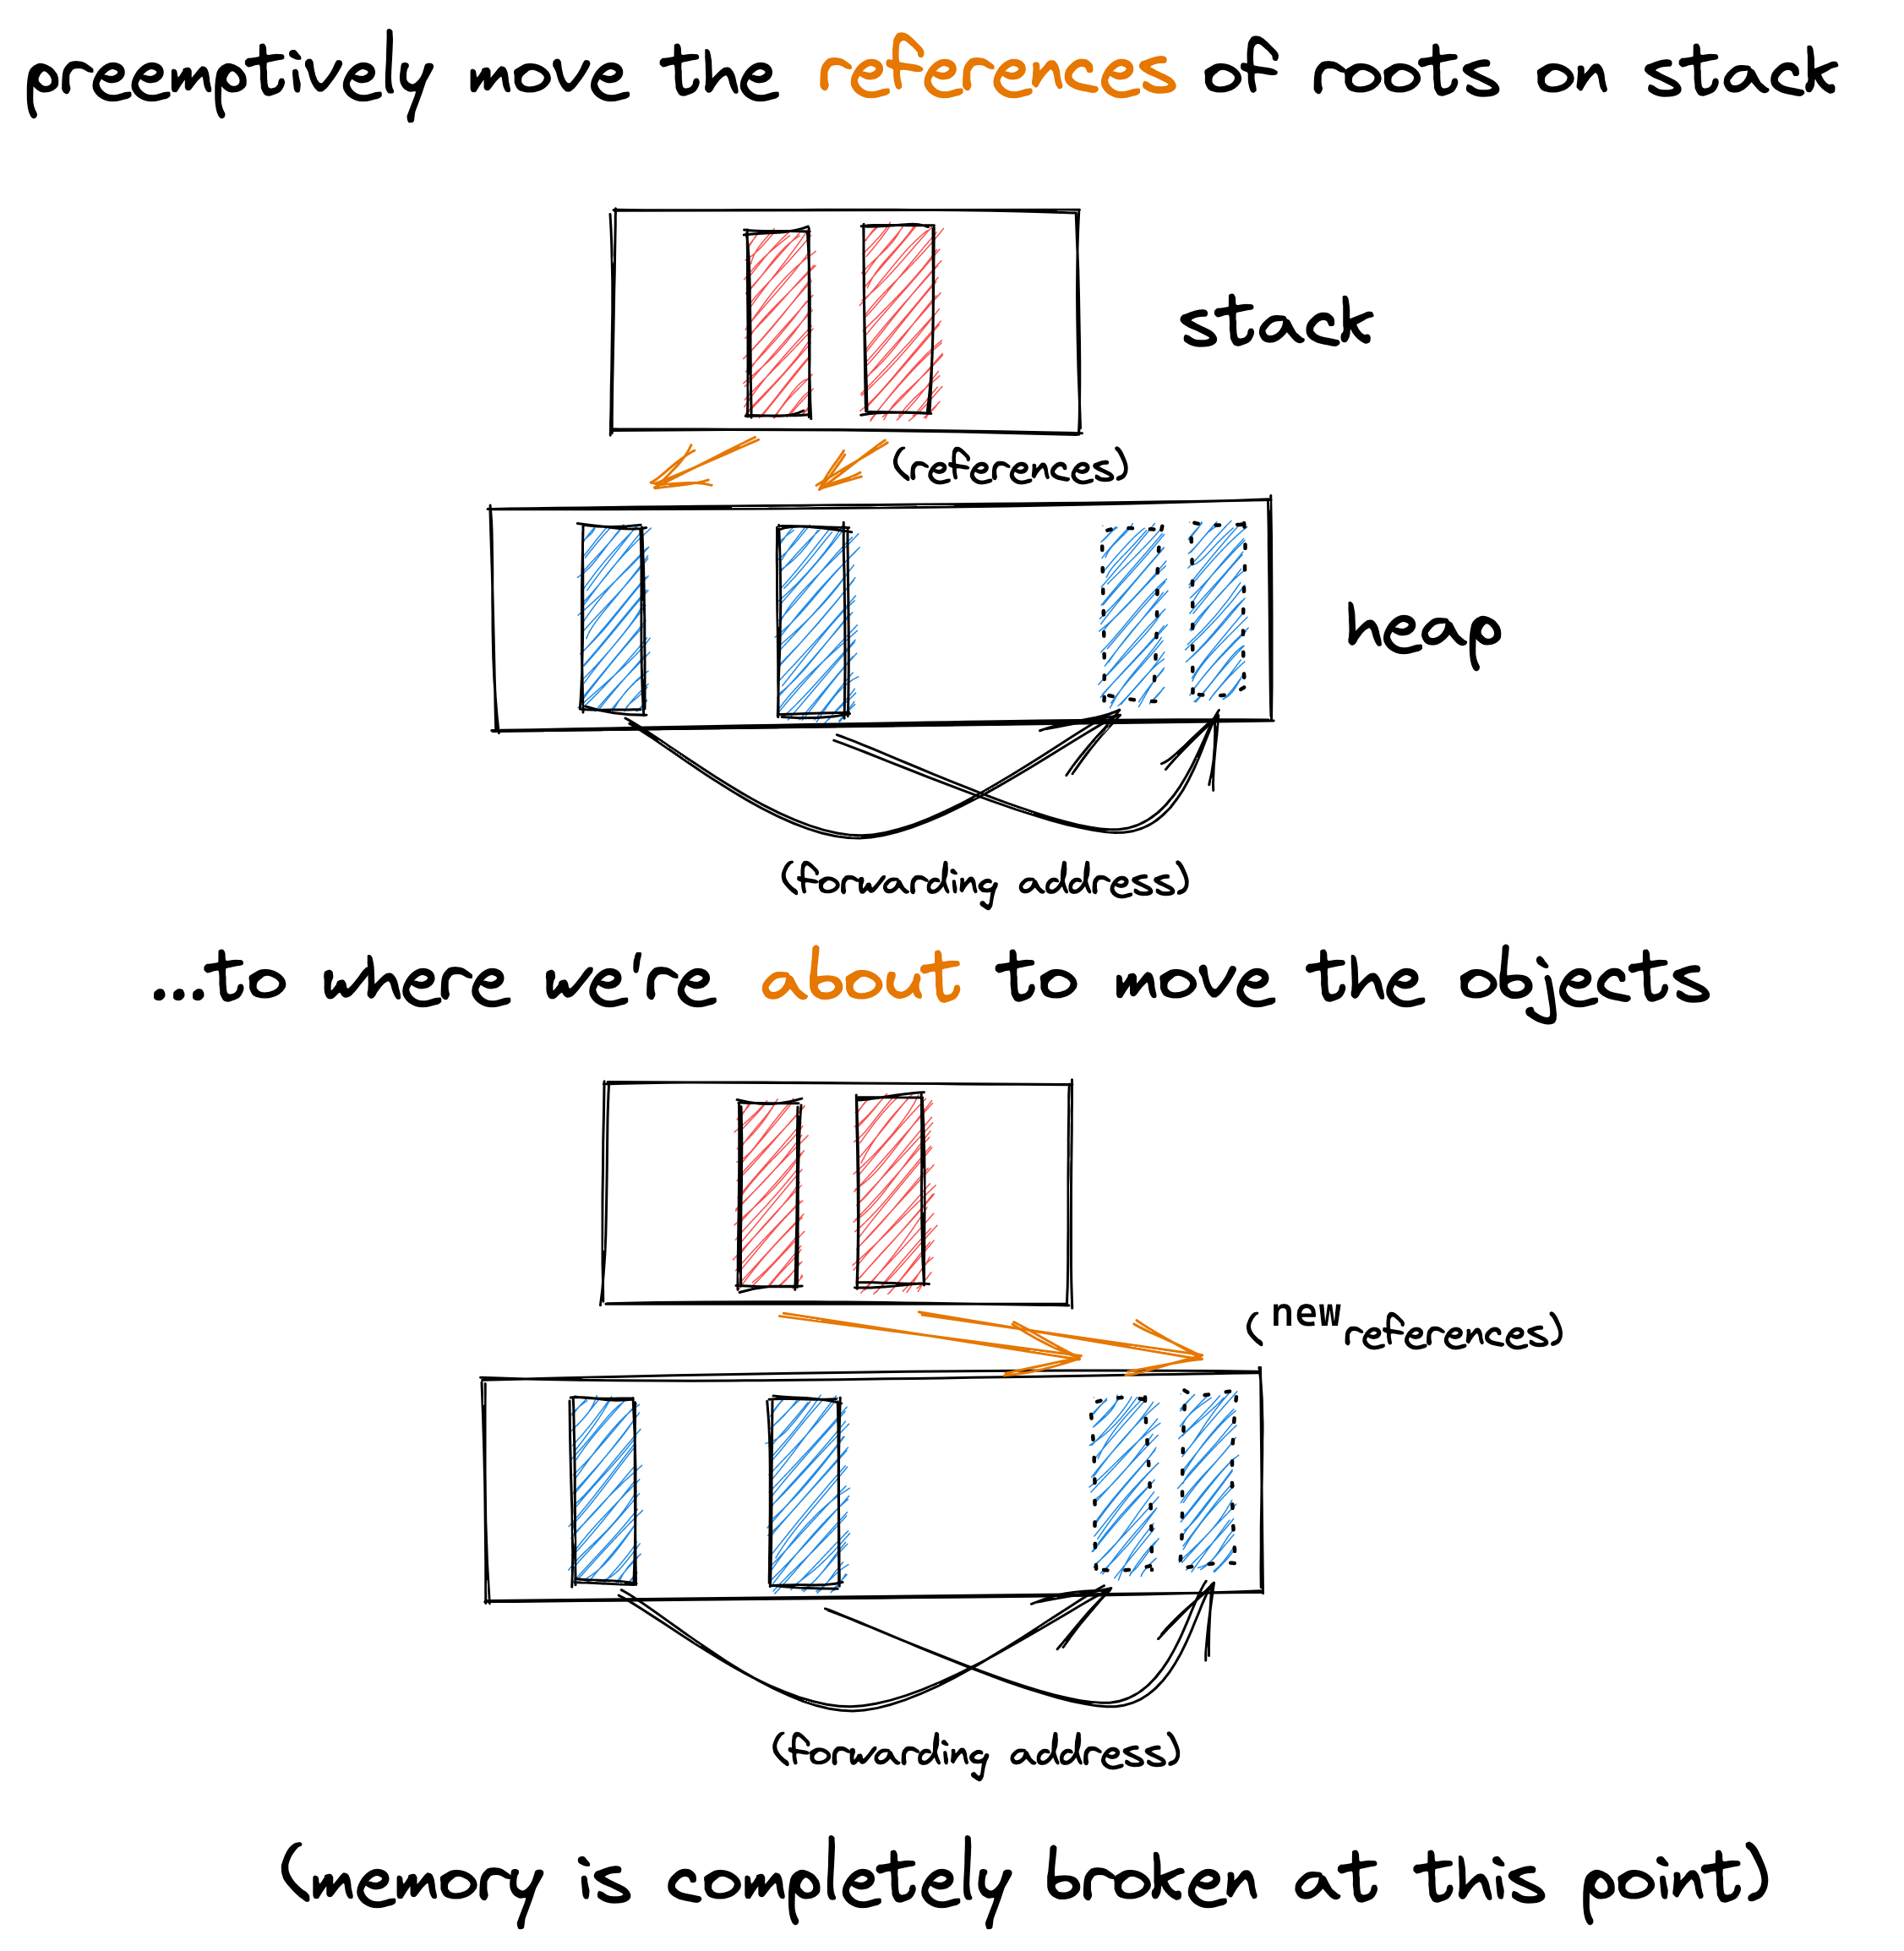
\includegraphics[scale=0.3]{pics/update-references.png}
    \caption{Updating references in the compact step of mark compact, visualized.}
\end{figure}

Finally, we move the objects over to where their \verb+forwarding_address+ points to

\begin{figure}[H]
    \centering
    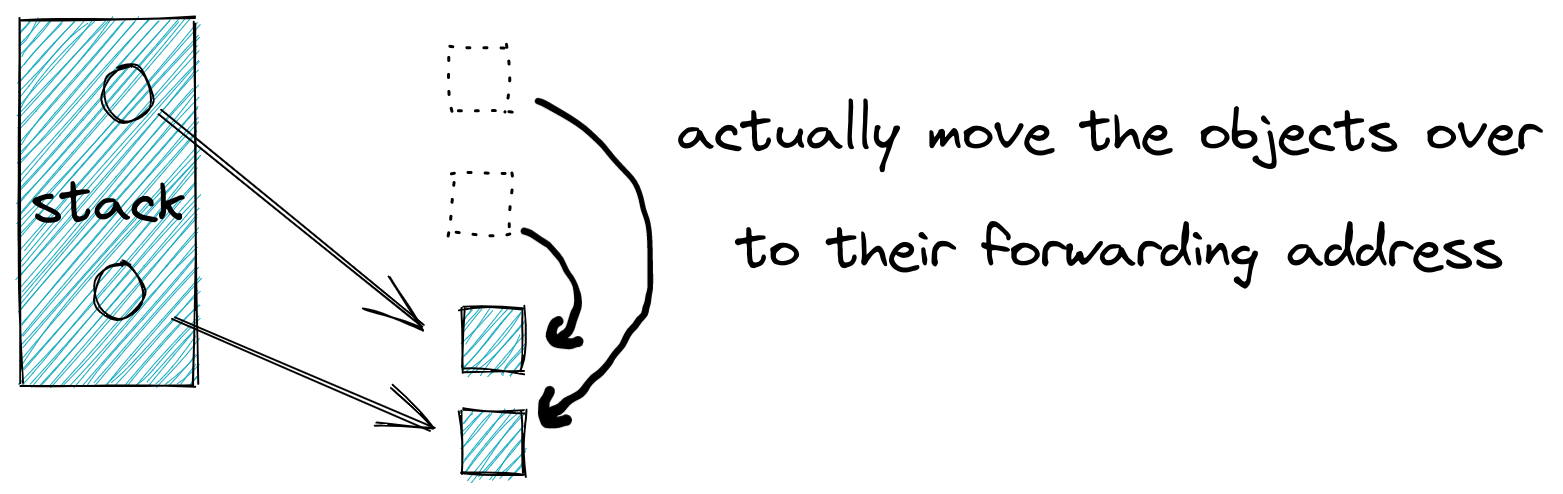
\includegraphics[scale=0.25]{pics/actually-move.png}
    \caption{Actually moving objects, the ``compact step'' in the compact step of mark compact, visualized.}
\end{figure}

Traverse the marked objects in the heap a 3rd time, then make \mintinline{rust}{std::mem::swap} calls between where the object is currently located and their \verb+forwarding-address+. It should be noted that the sliding mark-compaction algorithm \textit{maintains the order} of which the objects were inserted in the original heap. It also moves objects \textit{more closely together} towards the front end of memory, which is why the LISP-2 algorithm is known as a ``sliding'' mark-compact algorithm.

The order of compacted objects is an important distinction to make in comparing the LISP-2 and Cheney's algorithms because Cheney's does not preserve the order of objects in memory.

\subsection{Cheney's Stop-and-Copy Algorithm}

The second type of garbage collector is Cheney's stop-and-copy algorithm. This algorithm uses double the memory of the LISP-2 mark-compact algorithm, but in return, is able to both mark and copy objects in one pass of the live objects.

When initializing the heap, we split it into two sections, which we call \verb+from_space+ and a \verb+to_space+~\parencite[Chapter~2]{gc_handbook}.

\begin{figure}[H]
    \centering
    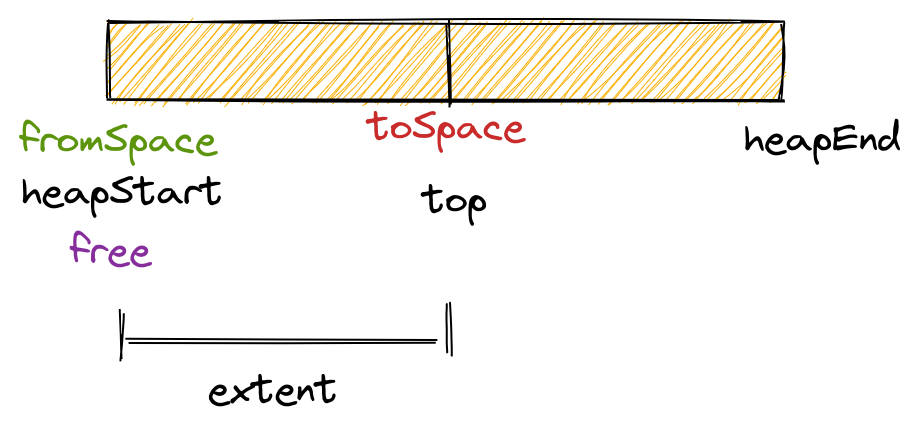
\includegraphics[scale=0.3]{pics/split-heap-diagram.png}
    \caption{Picture of what the heap looks like for a stop-and-copy algorithm}
\end{figure}

Like the mark-compact algorithm, on every allocation, we check if the heap has enough free space by attempting to bump the \verb+free+ pointer and check if it's less than the \verb+top+ of the heap.

\begin{figure}[H]
    \centering
    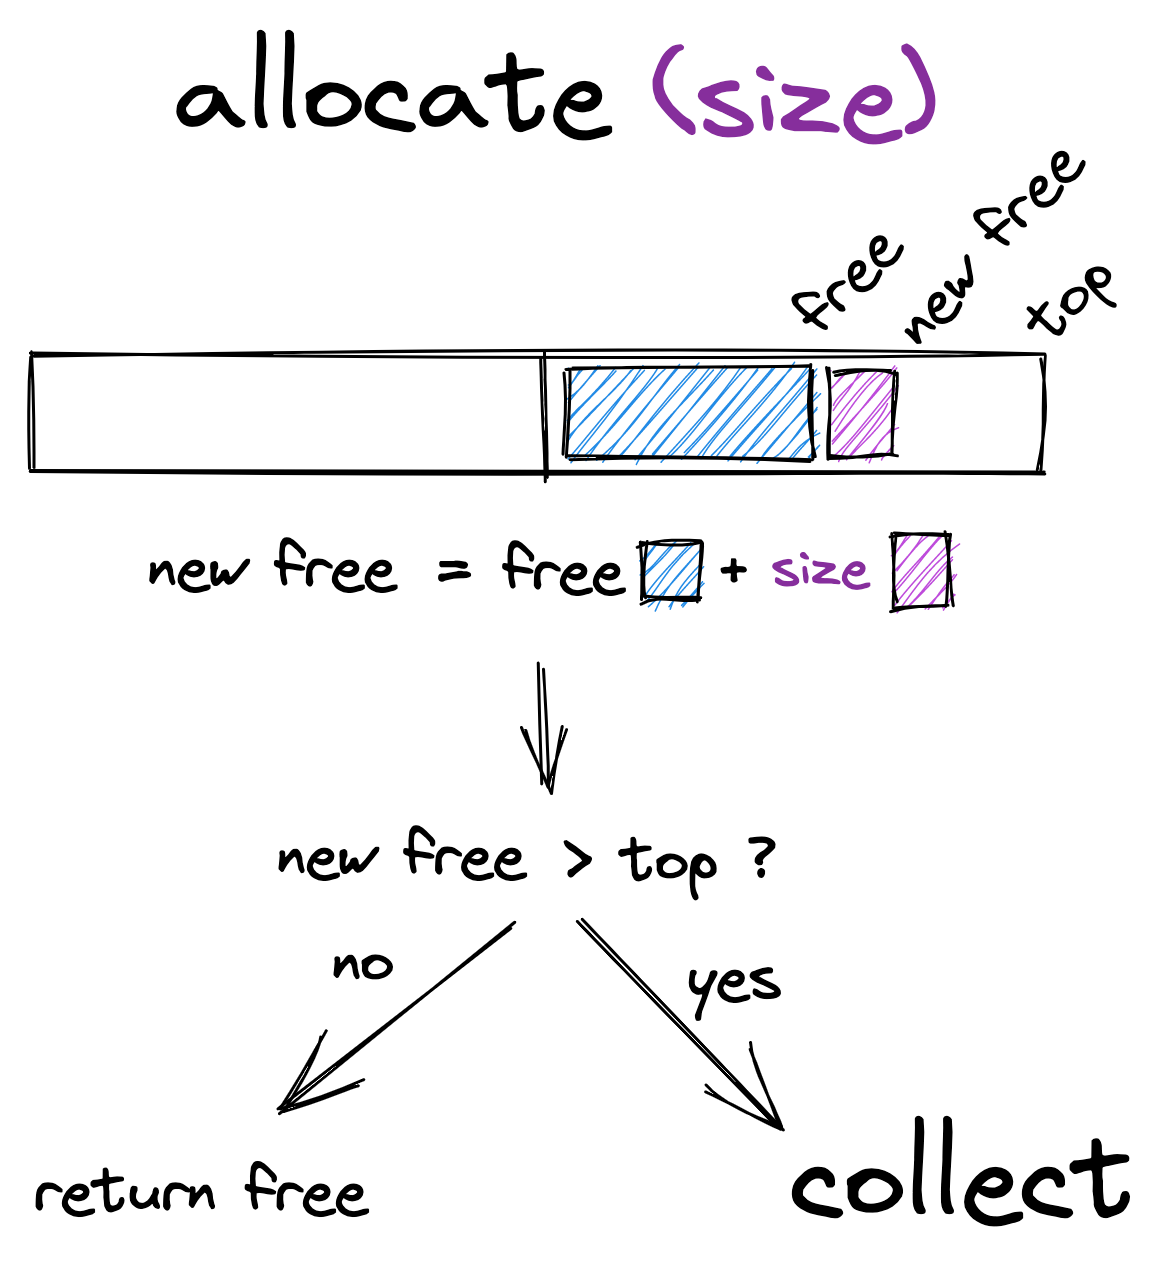
\includegraphics[scale=0.3]{pics/allocation.png}
    \caption{What checking for allocations looks like.}
\end{figure}

In this case, because the heap is split in half, we check that the \verb+free+ is not greater than the end of the heap but rather that it is not greater than half of the size of the heap. Once the heap does end up filling up, we can no longer allocate a new object on the heap and thus must call the \verb+collect()+ function.

\subsubsection{Cheney's Algorithm}

Right as the \verb+collect()+ function is called, we flip the \verb+from_space+ with \verb+to_space+. 

\begin{figure}[H]
    \centering
    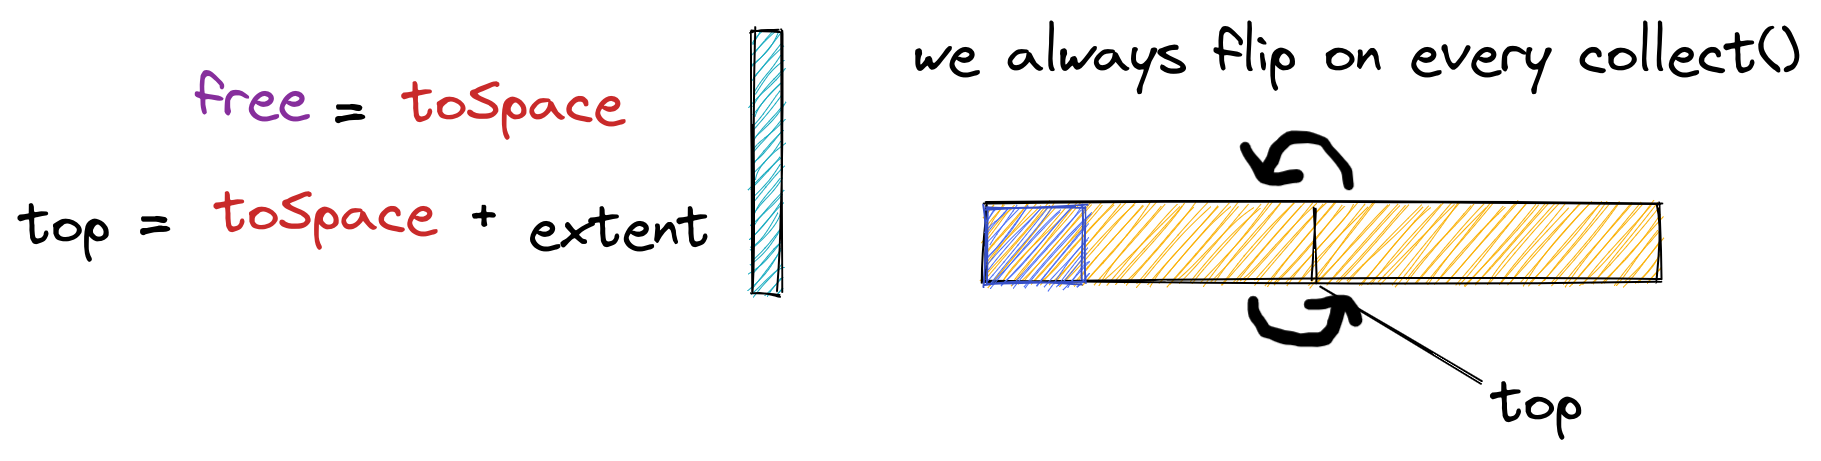
\includegraphics[scale=0.25]{pics/flipping.png}
    \caption{flipping}
\end{figure}

Then we follow that by \verb+copy+ing the initial children of the roots reachable by the program into \verb+to_space+. Note that the children moved into \verb+to_space+ still hold references that point to objects in \verb+from_space+.

Inside the \verb+copy+ function, we move the children of the roots over (if they haven't been moved already), then update the \verb+forwarding-address+ of their old location on \verb+from-space+ to point to their new location on \verb+to_space+.

\begin{figure}[H]
    \centering
    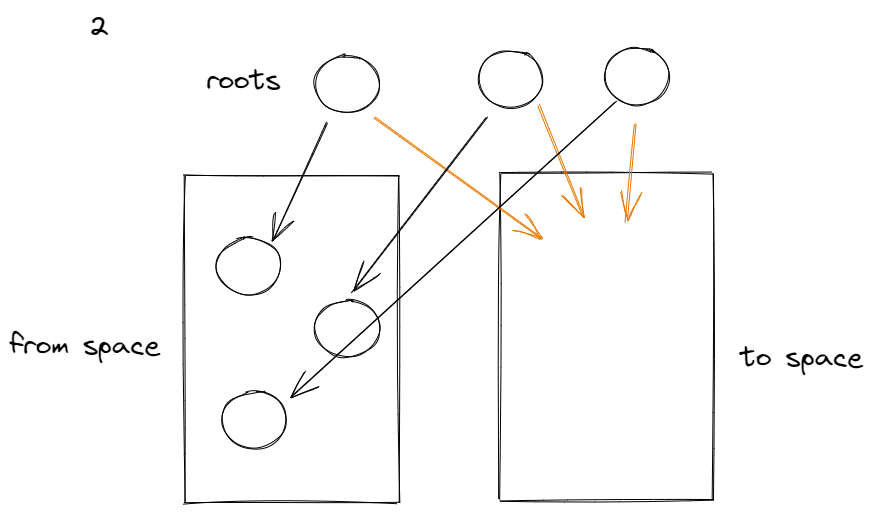
\includegraphics[scale=0.3]{pics/visualization-of-worklist.png}
    \caption{The algorithm for stop and compact. During the collect function, objects in from space are copied to to space, and their forwarding addresses are updated to point to the copied objects in to space.}
\end{figure}

Now, the objects and references of objects in \verb+to_space+ effectively act as a worklist. For every remaining object in \verb+to_space+ (including the roots that we just moved), we take the objects they reference, move them over to \verb+to_space+ if we haven't already, and then update the references to point to \verb+to_space+. (If their references have already been moved, then we can just use their \verb+forwarding_address+ that we updated on the \verb+from_space+ to point to the right location) 

It should be noted that because the objects in \verb+to_space+ act as a worklist, stop-copy is inevitably breadth-first. This is opposed to mark-compact, which gives us the freedom to choose between using a stack and queue (and therefore between breadth-first or depth-first) in the marking stage, and preserves insertion order in the move stage.

Upon reaching the end of the \verb+to_space+, garbage collection is done because all live objects have been copied to the effective heap. At this point, the \verb+from_space+ is basically ignored, and the \verb+to_space+ becomes the effective heap until the next cycle of garbage collection occurs.

\section{Experiment}

From the algorithms above, one can infer that for a garbage collector, or more specifically, compacting collectors, there are two places where pure performance can be measured.\footnote{Because objects are compacted in both algorithms, allocations are similarly fast. (This is not the case for other tracing garbage collection algorithms, like mark-sweep, where the performance of the mutator is potentially much worse.) In light of this fact, allocator and mutator performance will not be considered in this paper}. The first place is the \verb+collect()+ part of the algorithm when the graph of live objects is traversed, and objects are moved to their compacted points. The second is the program's runtime performance when the objects on the heap are being accessed after garbage collection.

\subsection{Method}

To test and compare these two algorithms, both were implemented as part of a library for the Rust programming language, a low-level programming language with comparable performance to C with its own novel model of memory management. Being implemented in a low-level programming language, the performance of the algorithms would not be subject to performance impacts of that language's garbage collector.\footnote{Snippets source code for the algorithms can be found in the Appendix, as they have been referenced throughout the paper. The full source code for the algorithm implementations, as well as this paper, can be found at \href{https://github.com/SpicyRicecaker/gc-representation-rs}{https://github.com/SpicyRicecaker/gc-representation-rs}}

To generate the testing data, a binary tree will be created with an arbitrary size of \(1,000,000\) objects.

Each node will be generated linearly via appending to a vector, with the indices representing pointers to memory addresses. Each parent node will have two child nodes, and added via \textit{breadth-first} recursion. This means that a full layer of the tree is filled with nodes before moving onto the next layer. 

Next, parents are then linked randomly to children using a seeded random generator. This makes the data structure slightly more dynamic than a binary tree and more representative of real objects in a program. A seeded number would allow for generated values to be consistent across algorithms and multiple trials, making test results more consistent and much more reproducible.

Depending on the program, there may be different amounts of dead and live objects when the heap is filled and collection needs to be called. In order to change the ratio of dead to living objects, nodes are removed randomly from the tree (at an arbitrary number of layers under the root, so the entire tree won't be deleted). Live nodes are counted, and a calculated ratio of dead to living objects is recorded after garbage collection to serve as the independent variable for the graphs below.

Finally, to measure the collection performance, for each heap of the two algorithms, \verb+collect()+ is run, and the time taken measured and recorded (via benchmark program discussed later).

To measure the runtime performance, the value of all nodes in the graph will be summed up. We do this by traversing the heap from the roots. There will be two traversals: one using breadth-first search and one using depth-first search. The time taken to complete these traversals will be recorded.

The testing framework used in this experiment will be the \verb+criterion+ crate. This crate automatically runs each function for a set amount of time in the beginning to prep the cache~\parencite{brookheislerAnalysisProcessCriterion}, which is especially relevant for garbage collection, as the way objects are arranged in memory will be different after garbage collection is run, which would affect the layout of objects in the cache. It also runs each test multiple times to reach a target runtime length, which increases the certainty in the average value that it returns for the time it took to complete the function~\parencite{brookheislerAnalysisProcessCriterion}.

\subsection{Data}
\begin{figure}[H]
    \centering
    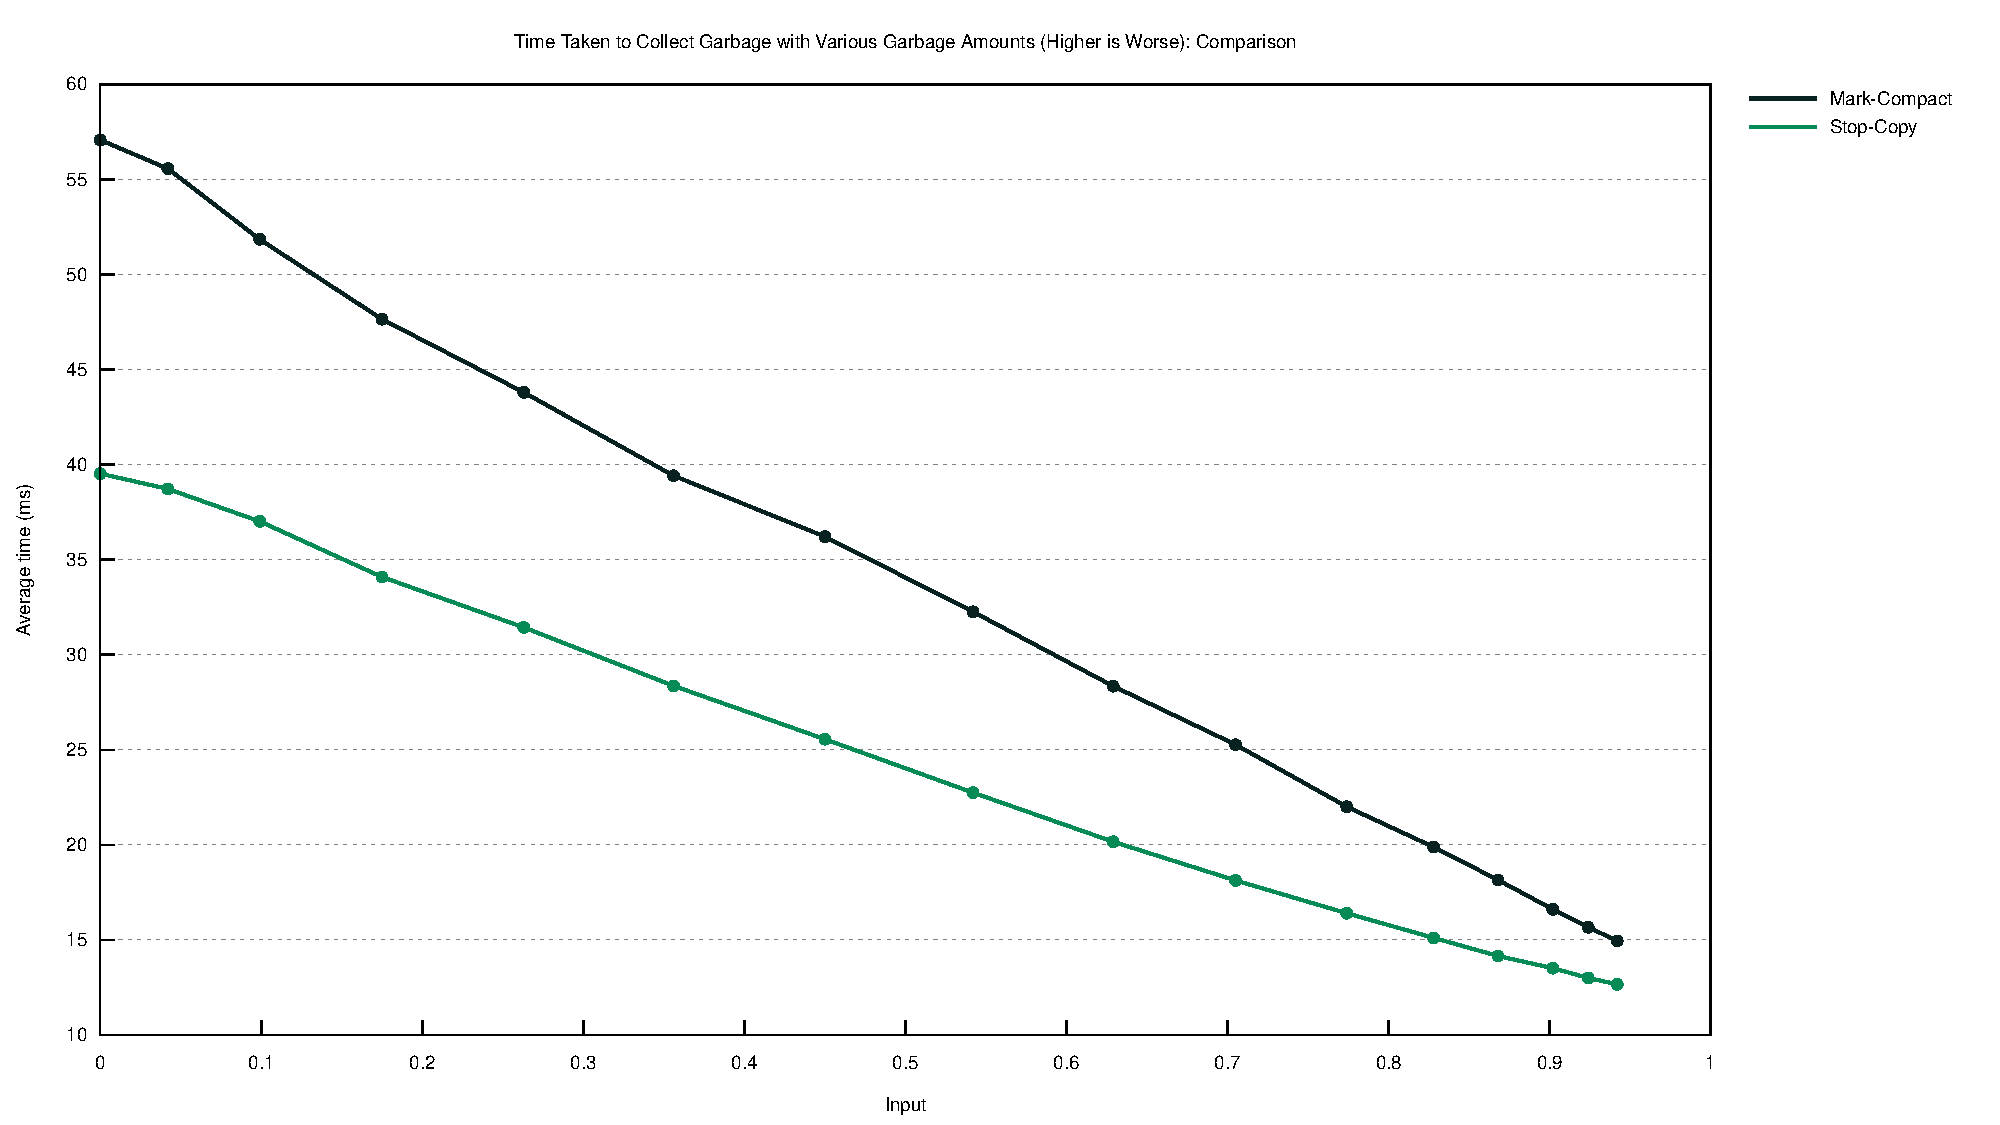
\includegraphics[width=0.91\textwidth]{pics/collect.pdf}
    \caption{Collection performance: Time Taken to Collect garbage with Various Garbage Amounts, where the \(x\)-axis demonstrates the ratio of dead to live objects in the heap before removal.}
\end{figure}
\begin{figure}[H]
    \centering
    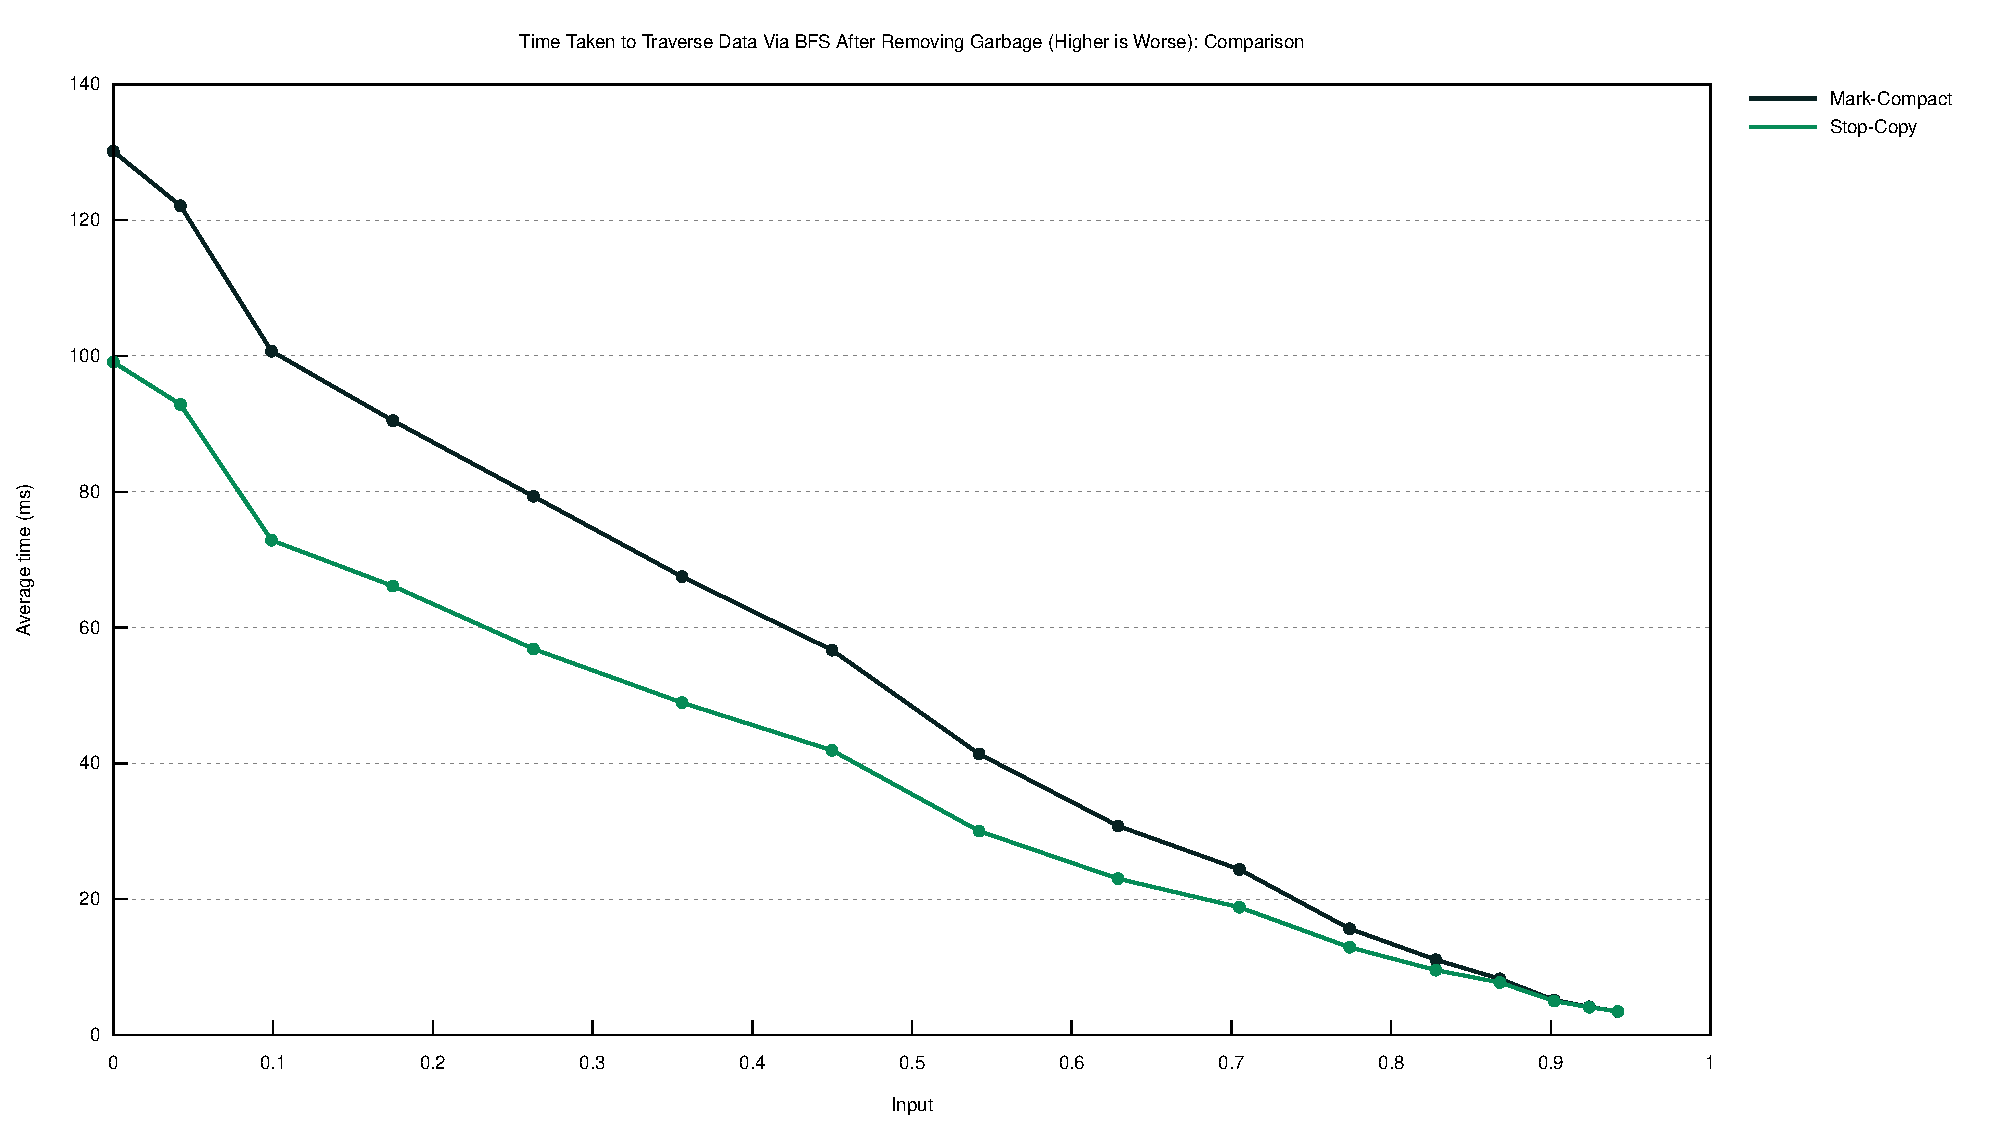
\includegraphics[width=0.91\textwidth]{pics/bfs.pdf}
    \caption{Runtime Performance: Time Taken to Traverse Data Via BFS after removing Garbage, where the \(x\)-axis demonstrates the ratio of dead to live objects in the heap before removal.}
\end{figure}
\begin{figure}[H]
    \centering
    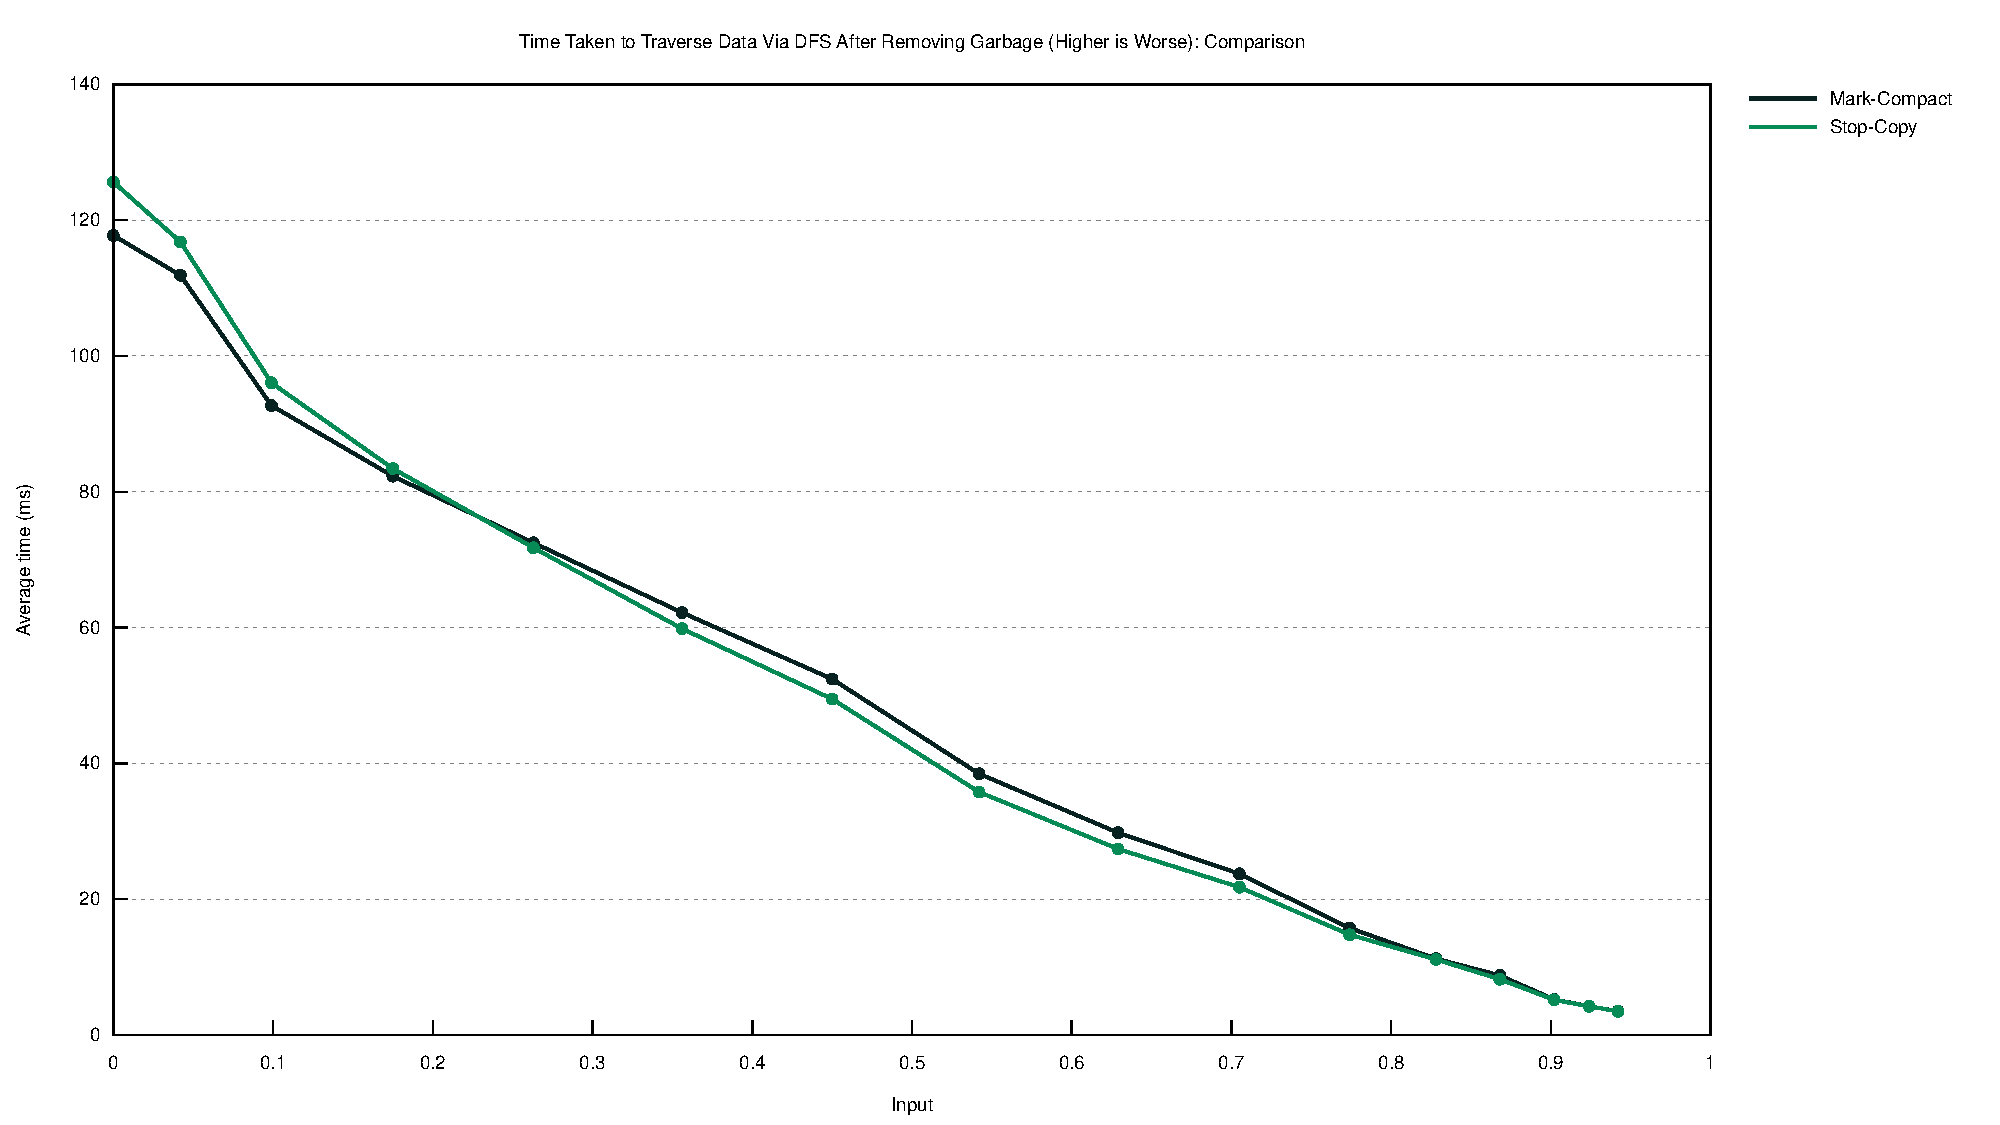
\includegraphics[width=0.91\textwidth]{pics/dfs.pdf}
    \caption{Runtime Performance: Time Taken to Traverse Data Via DFS after removing Garbage, where the \(x\)-axis demonstrates the ratio of dead to live objects in the heap before removal.}
\end{figure}

\begin{table}
    % the @{} removes minimal padding 
    % llr stands for left and right centering
    \centering
    \begin{tabular}{@{}ll@{}} \toprule
        Operating System & MacOs Montery 12.2 \\
        CPU               & Apple M1 Chip      \\
        RAM               & 8 Gb\\
        \bottomrule
    \end{tabular}
    \caption{Specs of the system used to benchmark the data}
\end{table}

\subsection{Observations and Analysis}

\subsubsection{Collection Performance}

Initially, with no garbage in a collection cycle, the collection performance of Cheney's algorithm is roughly \(1.4x\) as fast as the LISP-2 algorithm. This makes sense because the mark-compact algorithm had to traverse the heap three times, whereas Cheney's only had to traverse the heap once to determine the live and dead objects. However, Cheney's algorithm is not \(3x\) as fast as the LISP-2 style algorithm. This is perhaps because Cheney's algorithm had to \textit{copy every single} live object in the entire heap (as there were no dead objects) from \verb+from_space+ to \verb+to_space+ regardless of its current position, whereas the mark-sweep algorithm \textit{did not have to move any objects at all}. After all, objects were already in their compacted places for mark-sweep. Intuitively, copying memory around is fairly expensive.

Over time, however, the collection time of both algorithms trend down linearly, with the mark-compact collection algorithm having a consistently higher value in each iteration. This also makes sense because, for the stop-copy and mark-compact algorithms, the heap is only being traversed \(3n\) or \(n\) times, respectively. Therefore, decreasing the \(n\) should also impact the collection time linearly.

\subsubsection{Runtime Performance}

The runtime performance of the algorithms compared in Figure 9 show that even with no garbage objects, the stop-copy collector is faster by about 30 milliseconds compared to the mark-compact collector. This shows that simply by rearranging the order of objects in the heap and modifying nothing else, the runtime performance of the algorithms can change.

One possible explanation for this difference in the runtime performance of each algorithm purely from rearrangement of object order could be attributed to hardware.

Empirically, there have been two observations of the access of memory: one is known as \textit{temporal locality}, the tendency of memory accessed once more likely to be accessed again in a small time frame, and the other \textit{spatial locality}, the tendency of memory close to memory that has just been accessed having a greater chance of being accessed again~\parencite[18:21]{oracledevelopersCachingUnderstandMeasure2015}.

To boost performance in light of these observations, in modern computers, memory is constructed hierarchically~\parencite{simondevCanJavaScriptGo2021} around the CPU.\@ From fastest access and smallest size to slowest access and the largest size, memory is layed out as follows: the L1, L2, and L3 caches, then random access memory (RAM)~\parencite{simondevCanJavaScriptGo2021}. Because the L caches are small, they can only cache parts of memory from a CPU.\@ Whenever main memory is accessed, objects that are close together in a \textit{cache line} (which, in modern computers, are 64-bytes) are put into the L caches~\parencites{simondevCanJavaScriptGo2021}{code_project}. Then on subsequent passes, the CPU checks the caches one by one for data before resorting to the heap. It's known as a cache `hit' when the CPU finds the data it needs in one of the L caches, and a cache `miss'~\parencite{simondevCanJavaScriptGo2021} when the CPU has to go all the way to the main memory to find the information that it needs.

Aside from memory data, it is also important to consider memory addresses. In modern systems a range of virtual memory addresses map to a range of physical memory addresses on hardware~\parencites{code_project}[31:29]{oracledevelopersCachingUnderstandMeasure2015}. These are stored in tables, and a \verb+page+ lookup table is allocated for each address to link these virtual addresses to physical addresses. However, looking up these values is expensive in terms of performance, so physical hardware has a lookup cache, with around the last 500 pages stored in it, called the transition lookup buffer (TLB)~\parencites{code_project}[32:42]{oracledevelopersCachingUnderstandMeasure2015}. Therefore, similar to the caches of the CPU, the TLB is also a cache essential for performance.

In the context of garbage collection, the stop-copy algorithm moves objects in a \textit{breadth-first} manner. That is, siblings of the same layer in the binary tree will be placed right next to each other in the heap. Then, during traversal, because siblings are closer together, there is a greater chance that adjacent siblings and nodes of the same layer of the binary tree are within the same cache line, so there is a greater chance that accessing one sibling may cause the CPU to cache those objects in the L caches. This raises the chance of there being a cache ``hit'' the next time CPU requests the memory for the next sibling. With more cache hits, the stop-copy collector would be much faster than the mark-compact collector. 

As part of the method for generating the binary tree, nodes of the binary tree were linked to random places around the heap. Therefore, parents who originally referenced children directly in the layer below might then reference other nodes in a manner more similar to that of a graph data structure. So even though the mark-compact algorithm preserved the insertion order of the binary tree, which placed siblings next to each other, these locality bonuses mostly likely became much less prominent after random linking.

The hypothesis that caching is causing performance differences is furhter supported by Figure 10, which shows the runtime performance of a \textit{depth-first} traversal as opposed to a \textit{breadth-first} traversal. In this case, we can see that the noticeable performance difference between mark-compact and the stop-and-copy algorithm has all but disappeared. This makes sense because even though mark-compact places siblings close together, a \textit{depth-first} traversal would go from parent to child to child, and so on until the leaf node is reached, resulting in there being less of a probability that the right nodes will be cached after being accessed. This would incurr a multitude of expensive cache misses.

\section{Conclusion}

\subsection{Areas of Error}

The first and most obvious source of error in this paper was that there was only one type of input, which was a binary tree with some extra links and some deletions. This binary tree was built and traversed breadth-first, meaning that siblings were placed side to side. Therefore, the stop-copy collector had more affinity with the dataset after its moves and ran faster than the mark-compact collector, which might not be the case if the data was created \textit{depth-first}, as suggested by the second runtime performance graph.

The mark-compact worklist's initial marking worklist was also implemented with a queue, which meant that it would have a greater advantage with regards to collecting this specific data set than a mark-compact which was built with a stack worklist.

Data was also added and deleted from the heap at random. This might not be the case for a practical program, in which it has been observed that younger objects tend to have a greater chance of ``dying'' than older objects~\parencite{youtube_introductory_video}. Old objects that never move from their place or exist for the entire runtime of the program might favor the mark-compact algorithm more, which doesn't move objects that are already compacted in place, unlike the copying collector.

And, secondly, because the entire graph was traversed to test runtime performance, there were no distinctions between the relative frequency at which young and old objects are accessed. In a real program, there would be this distinction. Take an object created with object-oriented concepts in mind, for example. To get the nested field on this object, a user would have to reference the parent, then the child, then the field of the child. If the parent holds lots of children, the parent would naturally be accessed more than the children.

Another consideration is that both the mark compact collector and stop and copy collector had to essentially traverse a graph to mark the live objects during the collection phase. This means that as garbage collections build up over time, the impact on object layout will cause differences in collection performance. In this experiment, a fresh heap was cloned before collection algorithms were run, so this factor in collection performance wasn't considered.

\subsection{Future Considerations}

In conclusion, the performance difference between Cheney's stop-and-sopy collector and the LISP-2 Sliding mark-compact is dependent on the situation. If data is accessed or oriented in such a way that it uses breadth-first traversal, then Cheney's rearranging, which causes better locality of reference and only one-time traversal of the heap to make it an easy choice over the mark-compact collector. However, when data isn't oriented correctly, the runtime performance difference between Cheney's algorithm and the LISP-2 collector becomes almost negligible. Cheney's also uses double the amount of memory to operate on the same heap compared to the mark-compact algorithm, meaning that for environments with limited memory, the mark-compact's low memory usage may be a better deal than having faster collections.

\newpage

\raggedright{}
\printbibliography[heading=bibintoc]

\section{Appendix}
\appendix
\renewcommand{\thesubsection}{\Alph{subsection}}

\subsection{Marking Stage}
\begin{minted}[linenos, breaklines]{rust}
// this block contains the code to mark all reachable objects
{
    // first create a worklist, which is going to be a queue, since
    // we're doing breadth-first traversal
    let mut worklist: VecDeque<NodePointer> = VecDeque::new();

    // populate the worklist with children reachable from the roots
    for root in &stack.roots {
        for child in &root.children {
            worklist.push_back(*child);
        }
    }

    // then we just keep on taking from the worklist until it's empty
    while let Some(node) = worklist.pop_front() {
        // if the node isn't marked (already)
        if !self.is_marked(node) {
            // we mark it because it means it's accessible
            self.mark(node);
            // then add the rest of its children to the back of the queue
            for child_node_pointer in &self.get(node).unwrap().children {
                worklist.push_back(*child_node_pointer);
            }
        }
    }
}
// now all our reachable objects should be marked, everything that isn't is
// considered garbo. We only care about the marked objects in our traversals
// from now on
\end{minted}
\subsection{Calculate Forwarding}
\begin{minted}[linenos, breaklines]{rust}
// the next three blocks contain the compact code
// free starts at 0, the beginning of the point which we wish to compact to
let mut free = 0;

// 1. the first step is to calculate new locations of all objects
{
    // we iterate over all objects in the heap
    for idx in 0..self.free {
        // if it is marked,
        if self.is_marked(idx.into()) {
            // set its forwarding address equal to free
            self.set_forwarding_address(idx.into(), free.into());
            // then bump free by the object's size
            free += 1;
            if free > self.committed_memory.len() {
                return Err("not enough space on heap to allocate new object. Something went wrong with marking objects in `collect()`".into());
            }
        }
    }
}
\end{minted}
\subsection{Update References}
\begin{minted}[linenos, breaklines]{rust}
// 2. the next step is to update object references
{
    // for every marked parent, set the parent's references to the
    // child's forwarding address
    for idx in 0..self.free {
        if self.is_marked(idx.into()) {
            let node = NodePointer::from(idx);

            //  for every child that the marked parent node holds
            for i in 0..self.get_mut(node).unwrap().children.len() {
                let child_node_pointer = self.get(node).unwrap().children[i];

                // get the child node's forwarding address
                let forwarding_address = self
                    .get(child_node_pointer)
                    .unwrap()
                    .forwarding_address
                    .unwrap();

                // then update the parent's reference to the child's forwarding address
                self.get_mut(node).unwrap().children[i] = forwarding_address;
            }
        }
    }
}
\end{minted}
\subsection{Move Objects}
\begin{minted}[linenos, breaklines]{rust}
// 3. actually move the objects
{
    //  for every marked node
    for idx in 0..self.free {
        if self.is_marked(idx.into()) {
            let node = NodePointer::from(idx);

            // unset the forwarding address of the object that's about
            // to be moved, consequently unmarking it for the next
            // collection cycle
            let forwarding_address = self.get(node).unwrap().forwarding_address.unwrap();
            self.get_mut(node).unwrap().forwarding_address = None;

            // swap node's current position with node's forwarding
            // position...  but only if they're not already in the right
            // place! This is an advantage of mark-compact over stop
            // copy
            if usize::from(forwarding_address) != usize::from(node) {
                self.committed_memory
                    .swap(usize::from(node), usize::from(forwarding_address));
            }
        }
    }
}
// set our new free pointer to the compacted point
self.free = free;
\end{minted}

\subsection{Cheney Allocations}
\begin{minted}[linenos, breaklines]{rust}
// allocates a new node to the heap
fn alloc(&mut self, node: Node, stack: &mut Stack) -> Result<NodePointer> {
    // check if free is going over fromspace + tospace
    if self.free >= self.top {
        log::trace!("exceeded from space, must run garbage collector");
        // we need to run gc
        self.collect(stack)?;
    }
    if self.free >= self.top {
        return Err("gg collection didn't result in any amount of garbage collected".into());
    }

    // set the node id to where the top of the heap is
    let node_pointer = NodePointer::from(self.free);
    // add it to the heap
    self.committed_memory[usize::from(node_pointer)] = node;
    // bump the free pointer
    self.free += 1;

    Ok(node_pointer)
}
\end{minted}
\subsection{Cheney Swap}
\begin{minted}[linenos, breaklines]{rust}
    // first we swap from space with tospace
{
    std::mem::swap(&mut self.from_space, &mut self.to_space);
    // set free to be at the bot of the new to_space
    self.free = self.to_space;
    // set top to be to_space plus the extent
    self.top = self.to_space + self.extent;
}
\end{minted}
\subsection{Cheney's Initial Population Function}
\begin{minted}[linenos, breaklines]{rust}
// next we populate the initial "working list" with roots
{
    // copy the roots over
    // this technically adds them to the worklist
    for root in &mut stack.roots {
        for child in &mut root.children {
            // make sure to update the root refs to point in the right place
            *child = self.copy(*child)?;
        }
    }
}
\end{minted}
\subsection{Copy Function}
\begin{minted}[linenos, breaklines]{rust}
/// copy function
pub fn copy(&mut self, node_pointer: NodePointer) -> Result<NodePointer> {
    // if object has a forwarding address, it means that we've already moved it
    // over to to space, so we can just return its reference
    if let Some(forwarding_address) = self.get(node_pointer).unwrap().forwarding_address {
        Ok(forwarding_address)
    } else {
        // otherwise, like in the mark-compact algorithm, we calculate the
        // location of where this object should exist in to space by bumping the
        // free pointer.
        let new_node_pointer = NodePointer::from(self.free);
        // now we use `.swap()` to move nodepointer current location to its new
        // location free
        self.committed_memory
            .swap(usize::from(node_pointer), usize::from(new_node_pointer));

        // and remember to set the forwarding address of the moved nodepointer
        // to none. This effectively unmarks it in preparation for the next
        // `collect()` cycle, similar to what we do in the mark compact
        // algorithm.
        self.get_mut(new_node_pointer).unwrap().forwarding_address = None;

        // now update the old forwarding address to include itself. This
        // effectively 'marks' the object to make sure that it isn't copied over
        // again. Keep in mind that this object in to space is basically
        // complete garbage except for its forwarding address part
        self.get_mut(node_pointer).unwrap().forwarding_address = Some(new_node_pointer);

        // also remember to bump the free pointer, as we just effectively
        // allocated something to `to_space`
        self.free += 1;

        // finally, we can return the new_node_pointer
        Ok(new_node_pointer)
    }
}
\end{minted}
\subsection{Copy Remaining}
\begin{minted}[linenos, breaklines]{rust}
    // now we process all the references of the nodes in the worklist as well
    {
    // you might be wondering...  how do we do `for each node in worklist`?
    // 
    // well, so long as the scan does not catch up to free that is, so as long
    // as we have not processed every single "copied" oject on the heap, keep on
    // going
    while scan < self.free {
        let scan_node_pointer = NodePointer::from(scan);
        // get all references, or children of the object that was recently
        // copied to tospace
        for i in 0..self.get(scan_node_pointer).unwrap().children.len() {
            // set the reference to whatever the forwarding address stored
            // inside the reference is, or copy it
            // 
            // now the reference should now be pointing to copied objects in tospace no matter what
            self.get_mut(scan_node_pointer).unwrap().children[i] =
                self.copy(self.get(scan_node_pointer).unwrap().children[i])?;
            // the references get added to the worklist automatically
        }
        // don't forget to bump the scan pointer
        scan += 1;
    }
}
\end{minted}


\end{document}